\documentclass[11pt,a4paper]{article}
\usepackage{amsmath}
% \usepackage[english]{babel}
\usepackage{graphicx}
\usepackage{picture}
\usepackage{color}
\usepackage{graphpap,color}
\usepackage{subfig}
\usepackage[percent]{overpic}

\usepackage[english]{babel}
\usepackage{amsfonts}
\usepackage{amssymb}
\usepackage{makeidx}
%\usepackage[usenames,dvipsnames,svgnames,table]{xcolor}
\definecolor{kuleuven}{RGB}{29,141,176}
\definecolor{kuleuven1}{RGB}{82,189,236}
\usepackage{geometry}

\newcommand{\nocontentsline}[3]{}
\newcommand{\tocless}[2]{\bgroup\let\addcontentsline=\nocontentsline#1{#2}\egroup}

\makeindex
\begin{document}

  % \frontmatter
  \newgeometry{textwidth=540pt,textheight=780pt,top=20pt,left=20pt,right=20pt}
  \begin{titlepage}

    \begin{figure}[t]{%
      \begin{overpic}[width=1\textwidth,natwidth=50,natheight=0]{Picture1.png}
        \put(46,4){\color{white}\large{\textbf{FACULTY OF ECONOMICS AND BUSINESS}}}
      \end{overpic}
      }
    \end{figure}

    \vspace*{4.5cm}
    {\color{kuleuven1}{\Huge  Feasibility of blockchain application \\as medium for collaborative systems or databases}}

    \vspace*{0.5cm}
    {\Large Researchplan}

    \begin{figure}[b]
      %\centering
      \begin{minipage}[c]{0.4\textwidth}  {%
        \begin{overpic}[width=0.9\textwidth,natwidth=300,natheight=370]{Picture2.png}
          \put(70,45){\begin{minipage}[c]{1.80\textwidth}
          \begin{flushright}

            {\Large Pelle Jacobs} \linebreak
            {r0364018} \linebreak

            {\large Masters in Information Systems Engineering}\linebreak
            {\large Majoring in Data Science}\linebreak
            \linebreak
            \textbf{{\large Promotor:}}   Prof. Dr. Jochem De Weerdt \linebreak
            \textbf{{\large Assistant:}} Vytautas Karalevicius
            \linebreak

            \textbf{{\large Academic year:}} {\large 2016-2017}
            \linebreak
          \end{flushright}
        \end{minipage}}
      \end{overpic}
      }
    \end{minipage}


    \begin{picture}(540,0.2)
      \put(0,0){\colorbox{kuleuven1}{\makebox(540,0.2){}}}
    \end{picture}
  \end{figure}

\end{titlepage}
%%%%%%%%%%%%%%%%%%%%%%%%%%%%%%%%%%%%%%%%%%%%%%%%%%%%%%%%%%%%%%%%%%%%%%%%%%%%%%%%%%%%%%%%%%%%%%%%%%%%
\restoregeometry
\setcounter{equation}{1}
\pagestyle{empty}

\tableofcontents
\pagebreak


%%%%%%%%%%%%%%%%%%%%%%%%%%%%%%%%%%%%%%%%%%%%%%%%%%%%%%%%%%%%%%%%%%%%%%%%%%%%%%%%%%%%%%%%%%%%%%%%%%%%%%%%%

My research into the Feasibility of blockchain application as medium for collaborative systems or databases will be split into three parts.

In the first part, I will focus on the concept of blockchain: what exactly do we define as blockchain and how does it work? What are other implementations of distributed ledger technology? What are the possibilities, advantages and disadvantages of blockchain?

After this analysis, I will switch to the other main topic of this thesis: collaborative systems and databases. Focussing on both distributed databases as decentralized databases, I will analyse their issues and investigate how current solutions try to solve these issues.

Finally, both these analyses will be combined in the final part, trying to formulate a framework that can evaluate the feasibility of blockchain on specific issues.

\section{What is blockchain and how is it used}

\subsection{Definition of 'blockchain'}

When starting a meaningful conversation about blockchain, it is never a bad idea to first come together on the definition of certain words, the concept of blockchain being one of the most important. Some people interprete blockchain as any distributed ledger, while for others the blockchain is strictly applicable to a ledger system as used by Bitcoin, including its many protocols. The definition used in this paper will probably be somewhere in between.

It will be important to clearly define the vocabulary, to avoid any misunderstanding further down the thesis. By defining blockchain, I will also be touching on the more general concept of 'distributed ledger technology', to make a clear difference.

\subsection{What does blockchain include}

After setting the scene, we will dive deeper into what the actual possibilities are of blockchains. In this chapter, I will be examining all the different implementations and uses of blockchains, going from private, permissioned blockchains to public, unpermissioned blockchains, from blockchains making use of the "proof of work" concept or to ones with the "proof of stake" concept, elaborating on the different types of data that can be stored on a blockchain and more specific, trying to give a deeper peek into the possibilities of smart contracts.

\subsection{Advantages and disadvantages of blockchain}

After thorough research of the possibilities, I will use the final chapter of this part to investigate the different advantages and disadvantages of the several possibilities of blockchains.

\subsection{Literature}

As blockchain is a very young field of research, most of the literature available still starts from the concept of Bitcoin. Besides several online articles, here are some of the books / papers on the study list:

\subsubsection{"Bitcoin: A Peer-to-Peer Electronic Cash System"}
S. Nakamoto, "Bitcoin: A Peer-to-Peer Electronic Cash System", 2008: The legendary paper by the mysterious Satoshi Nakamoto is what made this entire revolution start, and therefore a logical starting point.

\subsubsection{"Mastering Bitcoin"}
A. M. Antonopoulos, "Mastering Bitcoin", 2015: This conclusive, community driven bitcoin manual has meanwhile been published by O'Reilly, and is generally considered as one of the most conclusive introduction to the blockchain world.

\pagebreak
\section{Collaborative databases}

In the second part, a similar approach will be repeated to analyse the subject of collaborative databases: define a context of collaborative databases, investigate the problems with these types of databases and investigate which solutions currently exist.

\subsection{Which databases are collaborative?}
\begin{figure}[h]
  \centering
  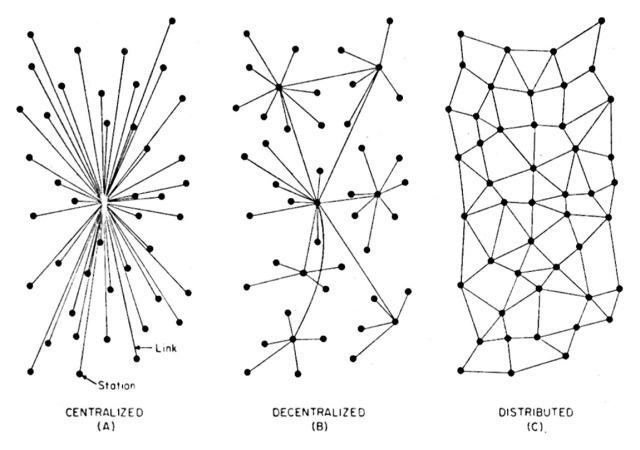
\includegraphics[width=.65\textwidth]{networktypes.jpg}
  \caption{Different collaborative network types. (P. Baran, "On Distributed Communication Networks", 1964)
  }
  \label{fig:networktypes}
\end{figure}

According to Baran (1964), there are generally three collaborative network types: centralized, decentralized, and distributed. To put it simply in the context of databases:
\begin{itemize}
  \item a centralized database has one main node with all the data to which several leafs (stations) are connected.
  \item a decentralized database has several main nodes that need to communicate to provide the correct data to the stations connected to this node. When one node fails however, the leafs connected to this node will (temporarily) not have access to the main data. A nice example would be Facebook, which has its data duplicated across several databases to ensure redudancy.
  \item in a distributed database, every leaf will function as a node that has a copy of the data, resulting in a network with an unlimited amount of nodes who not necessarily actually trust each other. The perfect example is of course Bitcoin.
\end{itemize}

As decentralized databases and distributed databases have more challenging issues, I will probably focus the rest of this paper on these two types.

\subsection{Current issues with collaborative databases}

Next, I will have a look at all the issues that distributed and decentralized databases face. Here are some issues that will probably be addressed:

\begin{itemize}
  \item Consistency: What is the truth? When data is not longer in one place, there is a need to determine the truth. For decentralized databases, this will consist of a method to synchronize several database instances. For distributed databases, this will be even more tricky, as the agents in the network can not necessarily be trusted. Therefore, there is need to somehow come to a consensus between the agents.
  \item Structure: complex databases will result in complex and unwieldy structures.
  \item Integrity and authenticity: How is made sure the data in the database is actually correct and authentic? How do we make sure no data disappears or gets maliciously altered?
\end{itemize}

\subsection{Current solutions}

As final chapter in this part, I will look into several solutions that currently try to solve these issues. One solution that very probably will be addressed is Cassandra from Facebook, a database management system designed to keep data synchronized between several servers.

\pagebreak

\section{Feasibility of blockchain application as medium for collaborative databases}
In the final part of the thesis, I will combine the previous two parts to answer the main research question: when can the potential of blockchain be leveraged to be a feasible solution for a collaborative database?

\subsection{Framework to evaluate feasibility of blockchain}
In this chapter, I will formulate a framework to evaluate the potential of blockchain for a specific issue based on simple questions, or to suggest a valuable alternative.

\subsection{Application of the framework on real world examples}
Finally, I will test this framework by applying it to several real world examples: "Was / is it a good idea to use blockchain in this specific use case?"

A popular, wide-spread hypothesis I am looking forward to evaluating: "The true power of blockchain lies in new issues that haven't been solved yet, instead of trying to replace current working solutions", the idea being that blockchain should rather be used for problems we are not solving yet, instead of trying to force blockchain as a solution to a problem it is not competent at solving. An analogy with the Internet is striking: while several companies tried (and failed) to force the internet as a solution to existing solutions (eg. pets.com for petfood shops), the true power of the Internet was revealed eg. when a student at Harvard thought it sounded fun to have his peers all connected on one website.



% EMPTY FINAL PAGE

\newpage
\thispagestyle{empty}
\newgeometry{textwidth=540pt,textheight=780pt,top=20pt,left=20pt,right=20pt}
\begin{figure}[ht]
  \begin{flushright}
    
\includegraphics[width=0.5\textwidth,natwidth=310,natheight=10]{Picture3.png}
  \end{flushright}
\end{figure}
\vfill
\begin{picture}(550,40)
  \put(0,0){\colorbox{kuleuven}{\makebox(520,52){}}}
\end{picture}
\end{document}
